\chapter{Pixel incidence matrix}
\label{app:pixel-incidence-matrix}

In this chapter we present the pixel incidence matrix defined in the theory of discrete calculus and we propose a curvature-based model using this concept.

\section{Cellular grid model}

We restrict our analysis to the integer plan because it's where theory and application is developped in this thesis, but it can be extended to higher dimensions. In the plan $\mathbb{Z}^2$, we identify faces (pixels), edges (linels) and vertices (pointels). An arbitrary (however coherent) orientation is set for faces and edges. For example, we set faces counter-clockwise, vertical edges to point up and horizontal edges to point right (see figure).

\begin{definition}{Pixel incidence matrix}
	Let $\Omega \in \mathbb{Z}^2$ be a connected portion of the integer plan with $m$ faces and $n$ edges. The linel incident matrix $\mathbf{P} \in \mathbb{Z}^{n \times m}$ is a matrix in which each column $\mathbf{P} _j$ represents the incidence relations between face $j$ and the edges of the domain.
\end{definition}

A face is incident to an edge if the edge itself is part of the face's boundary and not incident otherwise. We say it is positive incident to an edge if besides incident, the face orientation  agrees with the orientation the edge, and negative incident in the case it doesn't agree.

\[
\mathbf{P} _{i,j} = \left\{ \begin{array}{ll}
	1, & \text{face $j$ is positive incident to edge $i$}\\
	-1, & \text{face $j$ is negative incident to edge $i$}\\	
	0, & \text{otherwise}
\end{array}\right.
\]

\begin{example}
	Consider a portion $\Omega$ of $\mathbb{Z}^2$ with $9$ faces ,$24$ edges and orientation as depicted in figures \ref{fig:cell-grid-indices} and \ref{fig:cell-grid-orientation}. 	
	
\begin{figure}[h!]
\center
\subfloat[\label{fig:cell-grid-indices}]{%
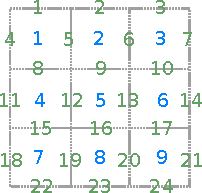
\includegraphics[scale=1]{figures/appendix-pixel-incidence-matrix/cell-grid-1.pdf}}\hspace{1em}%
\subfloat[\label{fig:cell-grid-orientation}]{%
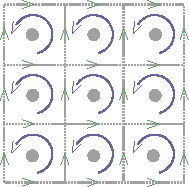
\includegraphics[scale=1]{figures/appendix-pixel-incidence-matrix/cell-grid-2.pdf}}\hspace{1em}%
\subfloat[\label{fig:cell-grid-active-pixels}]{%
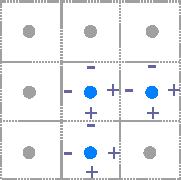
\includegraphics[scale=1]{figures/appendix-pixel-incidence-matrix/cell-grid-3.pdf}}\hspace{1em}%
\subfloat[\label{fig:cell-grid-active-linels}]{%
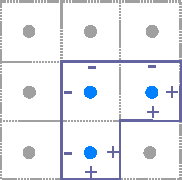
\includegraphics[scale=1]{figures/appendix-pixel-incidence-matrix/cell-grid-4.pdf}}%
\caption{Figures (a) and (b) illustrates indices assignments and orientation; figure (d) shows the result of applying the pixel incidence matrix for the active pixels in figure (c).}
\end{figure}

\[
   \begin{array}{ll}
	
	\mathbf{P} = \left[ \begin{array}{ccccccccc}
	 -1 & 0 & 0 & 0 & 0 & 0 & 0 & 0 & 0 \\
	 0 & -1 & 0 & 0 & 0 & 0 & 0 & 0 & 0 \\	 
	 0 & 0 & -1 & 0 & 0 & 0 & 0 & 0 & 0 \\	 
	 -1 & 0 & 0 & 0 & 0 & 0 & 0 & 0 & 0 \\	 
	 1 & -1 & 0 & 0 & 0 & 0 & 0 & 0 & 0 \\	 
	 0 & 1 & -1 & 0 & 0 & 0 & 0 & 0 & 0 \\	 
	 0 & 0 & 1 & 0 & 0 & 0 & 0 & 0 & 0 \\	 
	 1 & 0 & 0 & -1 & 0 & 0 & 0 & 0 & 0 \\	 
	 0 & 1 & 0 & 0 & -1 & 0 & 0 & 0 & 0 \\	 
	 0 & 0 & 1 & 0 & 0 & -1 & 0 & 0 & 0 \\	 
	 0 & 0 & 0 & -1 & 0 & 0 & 0 & 0 & 0 \\	 
	 0 & 0 & 0 & 1 & -1 & 0 & 0 & 0 & 0 \\	 
	 0 & 0 & 0 & 0 & 1 & -1 & 0 & 0 & 0 \\	 
	 0 & 0 & 0 & 0 & 0 & 1 & 0 & 0 & 0 \\	 
	 0 & 0 & 0 & 1 & 0 & 0 & -1 & 0 & 0 \\	 
	 0 & 0 & 0 & 0 & 1 & 0 & 0 & -1 & 0 \\	 
	 0 & 0 & 0 & 0 & 0 & 1 & 0 & 0 & -1 \\	 
	 0 & 0 & 0 & 0 & 0 & 0 & -1 & 0 & 0 \\	 
	 0 & 0 & 0 & 0 & 0 & 0 & 1 & -1 & 0 \\	 
	 0 & 0 & 0 & 0 & 0 & 0 & 0 & 1 & -1 \\	 
	 0 & 0 & 0 & 0 & 0 & 0 & 0 & 0 & 1 \\	 
	 0 & 0 & 0 & 0 & 0 & 0 & 1 & 0 & 0 \\	 
	 0 & 0 & 0 & 0 & 0 & 0 & 0 & 1 & 0 \\	 
	 0 & 0 & 0 & 0 & 0 & 0 & 0 & 0 & 1	 	 	 	 	 	 	 		\end{array}\right] &, \qquad
	 
	\mathbf{P} \left[ \begin{array}{l}
					0\\
					0\\
					0\\
					0\\
					1\\
					1\\
					0\\
					1\\
					0\\
					\end{array}\right] =  \left[ \begin{array}{l}
											0\\
											0\\
											0\\
											0\\
											0\\
											0\\
											0\\
											0\\
											-1\\
											-1\\
											0\\
											-1\\
											0\\
											1\\
											0\\
											0\\
											1\\
											0\\
											-1\\
											1\\
											0\\
											0\\
											1\\
											0
										\end{array}\right]
	 
   \end{array}
\]



The pixel incidence matrix applied for vector $\mathbf{x} \in \mathbb{Z}^9$, representing the active pixels depicted in figure \ref{fig:cell-grid-active-pixels}, results in vector $\mathbf{y} \in \mathbb{Z}^{24}$ representing the active boundary depicted in figure \ref{fig:cell-grid-active-linels}.

The linel incidence matrix is simply defined as the transpose of the pixel incidence matrix. Applying the former to a vector of active linels returns the set of incident pixels to the linels. For example, $\mathbf{P}^{T}\mathbf{P}$ applied to vector $x$ above results in $[0,-1,-1,-1,2,3,-1,3,-2]^T$. Positive coefficients represents inner incident pixels, and negative coefficients outer incident pixels. Moreover, the absolute value of each coefficient represents the number of linels incident to the corresponding pixel. For example, pixel $6$ is incident to three linels, namely the linels $10,14,17$.

\end{example}


\section{Numerical methods}

\begin{itemize}
	\item{Newton-Rapson}
	\item{Homotopy Continuation Method (Hom4PS-3)}
\end{itemize}


